\documentclass[finnish,english,t]{beamer}
%\documentclass[finnish,english,handout]{beamer}

\usepackage[T1]{fontenc}
\usepackage[utf8]{inputenc}
\usepackage{newtxtext} % times
%\usepackage[scaled=.95]{cabin} % sans serif
\usepackage{amsmath}
\usepackage[varqu,varl]{inconsolata} % typewriter
\usepackage[varg]{newtxmath}
\usefonttheme[onlymath]{serif} % beamer font theme
\usepackage{microtype}
\usepackage{epic,epsfig}
\usepackage{subfigure,float}
\usepackage{amsmath,amsfonts,amssymb}
\usepackage{inputenc}
\usepackage{babel}
\usepackage{afterpage}
\usepackage{url}
\urlstyle{same}
\usepackage{amsbsy}
\usepackage{eucal}
\usepackage{rotating}
\usepackage{listings}
\usepackage{lstbayes}
\usepackage{minted}
\setminted{highlightcolor=lightyellow}
\usepackage{natbib}
\bibliographystyle{apalike}

\mode<presentation>
{
  \setbeamercovered{invisible}
  \setbeamertemplate{itemize items}[circle]
  \setbeamercolor{frametitle}{bg=white,fg=navyblue}
  \setbeamertemplate{navigation symbols}{}
  \setbeamertemplate{headline}[default]{}
  \setbeamertemplate{footline}[split]
  % \setbeamertemplate{headline}[text line]{\insertsection}
  \setbeamertemplate{footline}[frame number]
}

\pdfinfo{            
  /Title      (BDA, Lecture 6) 
  /Author     (Aki Vehtari) % 
  /Keywords   (Bayesian data analysis)
}

\definecolor{lightyellow}{rgb}{1,1,0.878}
\definecolor{navyblue}{rgb}{0,0,0.5}
\renewcommand{\emph}[1]{\textcolor{navyblue}{#1}}
\definecolor{darkgreen}{rgb}{0,0.3922,0}

\makeatletter
\newcommand{\minted@style@bw}{%
  \renewcommand\fcolorbox[3][]{##3}%
  \renewcommand\textcolor[3][]{##3}%
  \color{gray}
}

% define new minted option "gray"
\minted@def@opt@switch{gray}
\fvset{formatcom*={%
  \ifthenelse{\equal{\minted@get@opt{gray}{true}}{true}}
  {\minted@style@bw}{}%
}}
\makeatother

\graphicspath{{./figs/}}

\parindent=0pt
\parskip=8pt
\tolerance=9000
\abovedisplayshortskip=2pt

\def\o{{\mathbf o}}
\def\t{{\mathbf \theta}}
\def\w{{\mathbf w}}
\def\x{{\mathbf x}}
\def\y{{\mathbf y}}
\def\z{{\mathbf z}}

\def\eff{\mathrm{eff}}
\def\ESS{\mathrm{ESS}}

\DeclareMathOperator{\E}{E}
\DeclareMathOperator{\Var}{Var}
\DeclareMathOperator{\var}{var}
\DeclareMathOperator{\Sd}{Sd}
\DeclareMathOperator{\sd}{sd}
\DeclareMathOperator{\Gammad}{Gamma}
\DeclareMathOperator{\Invgamma}{Inv-gamma}
\DeclareMathOperator{\normal}{normal}
\DeclareMathOperator{\Bin}{Bin}
\DeclareMathOperator{\Negbin}{Neg-bin}
\DeclareMathOperator{\Poisson}{Poisson}
\DeclareMathOperator{\Beta}{Beta}
\DeclareMathOperator{\logit}{logit}
\DeclareMathOperator{\N}{N}
\DeclareMathOperator{\U}{U}
\DeclareMathOperator{\BF}{BF}
\DeclareMathOperator{\Invchi2}{Inv-\chi^2}
\DeclareMathOperator{\NInvchi2}{N-Inv-\chi^2}
\DeclareMathOperator{\InvWishart}{Inv-Wishart}
\DeclareMathOperator{\tr}{tr}
% \DeclareMathOperator{\Pr}{Pr}
\def\euro{{\footnotesize \EUR\, }}
\DeclareMathOperator{\rep}{\mathrm{rep}}

\title[]{Bayesian data analysis}
\subtitle{}

\author{Aki Vehtari}

\institute[Aalto]{}

\begin{document}

\begin{frame}{Hamiltonian Monte Carlo and Stan}

  \begin{itemize}
  \item<+-> Hamiltonian Monte Carlo uses gradient information and dynamic
    simulation to reduce random-walk and increase acceptance rate
    \begin{itemize}
    \item the performance scales well with the number of dimensions
    \item this lecture introduces the basic HMC and No-U-Turn-Sampler
      based dynamic HMC
    \item other useful variants have been developed recently
    \end{itemize}
  \item<+-> Stan is the most popular probabilistic programming framework
    \begin{itemize}
    \item many recent probprog frameworks use dynamic HMC samplers
    \item this lecture introduces Stan language and main features
    \item later you can also use higher level packages built on top of
      Stan
    \end{itemize}
  \end{itemize}

\end{frame}

\begin{frame}{BDA Chapter 12}

  \begin{itemize}
  \item {\color{gray} 12.1 Efficient Gibbs samplers (not part of the course)}
  \item {\color{gray} 12.2 Efficient Metropolis jump rules (not part of the course)}
  \item {\color{gray} 12.3 Further extensions to Gibbs and Metropolis (not part of the course)}
  \item 12.4 Hamiltonian Monte Carlo (important)
  \item 12.5 Hamiltonian dynamics for a simple hierarchical model (useful example)
  \item 12.6 Stan: developing a computing environment (useful intro)
  \end{itemize}
\end{frame}

\begin{frame}{Extra material for HMC / NUTS}

  \begin{itemize}
  \item An introduction for applied users with good visualizations:\\
    Monnahan, Thorson, and Branch (2016)
    Faster estimation of Bayesian models in ecology using Hamiltonian
    Monte Carlo. \url{https://dx.doi.org/10.1111/2041-210X.12681}
  \item A technical review of why HMC works:\\
    Neal (2012). MCMC using Hamiltonian
    dynamics. \url{https://arxiv.org/abs/1206.1901}
  \item The No-U-Turn Sampler:\\
    Hoffman and Gelman (2014). The No-U-Turn
    Sampler: Adaptively Setting Path Lengths in Hamiltonian Monte
    Carlo. \url{https://jmlr.csail.mit.edu/papers/v15/hoffman14a.html}
  \item Multinomial variant of NUTS:\\
    Betancourt (2018).  A Conceptual Introduction to
    Hamiltonian Monte Carlo. \url{https://arxiv.org/abs/1701.02434}
  \end{itemize}

\end{frame}


\begin{frame}{Extra material for Stan}

  \begin{itemize}
  \item Gelman, Lee, and Guo (2015) Stan: A
    probabilistic programming language for Bayesian inference and
    optimization. \url{http://www.stat.columbia.edu/~gelman/research/published/stan_jebs_2.pdf}
  \item Carpenter et al (2017). Stan: A probabilistic programming
    language. Journal of Statistical Software
    76(1). \url{https://dox.doi.org/10.18637/jss.v076.i01}
  \item Stan User's Guide, Language Reference Manual, and Language
    Function Reference (in html and pdf)
    \url{https://mc-stan.org/users/documentation/}
    \begin{itemize}
    \item[-] easiest to start from Example Models in User's guide
    \end{itemize}
  \item Basics of Bayesian inference and Stan, part 1 Jonah Gabry \&
    Lauren Kennedy (StanCon 2019 Helsinki tutorial)
    \begin{itemize}
    \item[-]
      \url{https://www.youtube.com/watch?v=ZRpo41l02KQ&index=6&list=PLuwyh42iHquU4hUBQs20hkBsKSMrp6H0J}
    \item[-] \url{https://www.youtube.com/watch?v=6cc4N1vT8pk&index=7&list=PLuwyh42iHquU4hUBQs20hkBsKSMrp6H0J}
  \end{itemize}
  \end{itemize}
\end{frame}


\begin{frame}{Chapter 12 demos}

  \begin{itemize}
  \item demo12\_1: HMC
  \item \url{https://chi-feng.github.io/mcmc-demo/}
  \item \url{http://elevanth.org/blog/2017/11/28/build-a-better-markov-chain/}
  \item cmdstanr\_demo, rstan\_demo
  \item \url{http://sumsar.net/blog/2017/01/bayesian-computation-with-stan-and-farmer-jons/}
  \item \url{http://mc-stan.org/documentation/case-studies.html}
  \item \url{https://mc-stan.org/cmdstanr/}
  \item \url{https://mc-stan.org/rstan/}
  \end{itemize}
  
\end{frame}

\begin{frame}{Hamiltonian Monte Carlo}

  \begin{itemize}
  \item<+-> Originally for quantum-chromo-dynamic simulation (Duane et
    al., 1987)
  \item<+-> Radford Neal started using for Bayesian neural networks in 1990's
  \item<+-> The performance scales well with the number of dimensions
  \item<+-> Hoffman and Gelman's (2014) NUTS variant and step size
    adaptation made it more robust wrt the algorithm parameters and
    thus easier to use
  \item<+-> Stan was the first probabilistic programming framework
    using HMC+NUTS
  \item<+-> Now most popular probabilistic programming frameworks use
    it (Stan, PyMC, TFP, Pyro, Turing.jl, etc.)
  \item<+-> Also used as the a high-fidelity reference in Approximate
    Inference in Bayesian Deep Learning competition
    \url{https://izmailovpavel.github.io/neurips_bdl_competition/}
  \end{itemize}
  
\end{frame}

\begin{frame}{Hamiltonian Monte Carlo}

  \vspace{-0.5\baselineskip}
  \begin{itemize}
  \item Uses log density (negative log density is called energy)
  \item Uses gradient of log density for more efficient sampling
  % \item Augments parameter space with momentum variables
  \end{itemize}
  \vspace{-0.6\baselineskip}
  \only<1>{\phantom{\includegraphics[width=9cm]{hmcdemo01.pdf}}}
  \only<2>{\includegraphics[width=9cm]{hmcdemo01.pdf}}
  \only<3>{\includegraphics[width=9cm]{hmcdemo02.pdf}}
  \only<4>{\includegraphics[width=9cm]{hmcdemo03.pdf}}
  \only<5>{\includegraphics[width=9cm]{hmcdemo04.pdf}}
  \only<6>{\includegraphics[width=9cm]{hmcdemo05.pdf}}
  \only<7>{\includegraphics[width=9cm]{hmcdemo06.pdf}}
  \only<8>{\includegraphics[width=9cm]{hmcdemo07.pdf}}
  \only<9>{\includegraphics[width=9cm]{hmcdemo08.pdf}}
  \only<10>{\includegraphics[width=9cm]{hmcdemo09.pdf}}
  \only<11>{\includegraphics[width=9cm]{hmcdemo10.pdf}}
  \only<12>{\hspace{-5mm}\includegraphics[width=12cm]{hmc1trace.pdf}}
  \only<13>{\hspace{-5mm}\includegraphics[width=12cm]{hmc1acf.pdf}}
  \only<14>{\hspace{-5mm}\includegraphics[width=12cm]{hmc1mcerr.pdf}}
\end{frame}

\begin{frame}{Hamiltonian Monte Carlo / No-U-Turn sampling}

  \begin{itemize}
  \item<+->[1.] HMC basics (static HMC)
  \item<+->[2.] HMC + leapfrog discretization + Metropolis (static HMC)
    \begin{itemize}
    \item Duane et al. (1987)
    \end{itemize}
  \item<+->[3.] NUTS + slice sampling + Metropolis (dynamic HMC)
    \begin{itemize}
    \item Hoffman \& Gelman et al. (2014)
    \end{itemize}
  \item<+->[4.] NUTS + multinomial (dynamic HMC)
    \begin{itemize}
    \item Betancourt (2018)
    \end{itemize}
  \end{itemize}

\end{frame}

\begin{frame}{Hamiltonian Monte Carlo}

  \begin{itemize}
  \item Related methods
    \begin{itemize}
    \item<+-> Factorizing $p(\theta_1,\theta_2)=p(\theta_1 \mid \theta_2)p(\theta_2)$: sample from\\
      1) $p(\theta_2)$,\\
      2) $p(\theta_1 \mid \theta_2)$
    % \item<+-> Gibbs: sample from\\
    %   1) $p(\theta_2 \mid \theta_1)$,\\
    %   2) $p(\theta_1 \mid \theta_2)$
    \item<+-> Metropolis: jointly $p(\theta_1,\theta_2)$\\
      jump distribution is a combination of proposal distribution and
      point mass at the previous value
    \end{itemize}
  \item<+-> HMC
    \begin{itemize}
    \item Augment with $\phi$ (the same dimensionality as $\theta$)
    \item 1) sample directly from $p(\phi)$,\\
      2) make a special joint Metropolis step for $p(\theta,\phi)=p(\theta)p(\phi)$
    \end{itemize}
  \end{itemize}
  
\end{frame}

\begin{frame}{Hamiltonian Monte Carlo}

  \begin{itemize}
  \item[1)] Sample from $p(\phi)$
    \begin{itemize}
    \item define $p(\phi) = \normal(0,1)$
    \end{itemize}
  \item[2)] Metropolis update for $p(\theta,\phi)=p(\theta)p(\phi)$
    \begin{itemize}
    \item proposal from Hamiltonian dynamic simulation
    \end{itemize}
  
  \end{itemize}
  
\end{frame}

\begin{frame}{Hamiltonian dynamic simulation}

  \begin{itemize}
  \item Statistical mechanics and canonical distribution
    \begin{align*}
      p(\theta,\phi)&=p(\theta)p(\phi)\\
      &=\frac{1}{Z}\exp(-(U(\theta)+K(\phi)))\\
      &=\frac{1}{Z}\exp(-H(\theta,\phi))
    \end{align*}
    where
    \begin{itemize}
    \item $U$ is potential energy function
    \item $K$ is kinetic energy function
    \item $H$ is Hamiltonian energy function
    \item $\phi$ is called a momentum variable
    \end{itemize}
  \item<2-> The potential energy is the negative log density\\
    $U(\theta)=-\log(p(\theta))+C$
  \end{itemize}
  
  
\end{frame}

\begin{frame}{Hamiltonian dynamic simulation}

 Equations of motion, use also the gradient
  \begin{align*}
    \frac{d\theta_i}{dt} & = \frac{\partial H}{\partial \phi_i}\\
    \frac{d\phi_i}{dt} & = -\frac{\partial H}{\partial \theta_i}
  \end{align*}

  \includegraphics[width=10cm]{hmc_dynamics.png}\\
  {\footnotesize From Monnahan et al (2017)}
  
\end{frame}

\begin{frame}{Hamiltonian Monte Carlo}

  \begin{itemize}
  \item[1)] Sample from $p(\phi)$
    \begin{itemize}
    \item define $p(\phi) = \normal(0,1)$
    \end{itemize}
  \item[2)] Metropolis update for $p(\theta,\phi)=p(\theta)p(\phi)$
    \begin{itemize}
    \item proposal from Hamiltonian dynamic simulation $p(\theta,\phi) \propto \exp(-H(\theta,\phi))$
    \end{itemize}
  
  \end{itemize}
  \includegraphics[width=10cm]{hmc_dynamics.png}\\
  {\footnotesize From Monnahan et al (2017)}
  
\end{frame}

\begin{frame}{Leapfrog discretization}

  \begin{itemize}
  \item Leapfrog discretization
    \begin{itemize}
    \item preserves volume
    \item reversible
    \item discretization error does not usually grow in time
    \end{itemize}
  \end{itemize}
  {\includegraphics[height=5.5cm,trim=0 0 150 0,clip]{hmc_leapfrog.png}}
  \uncover<2>{\includegraphics[height=5.5cm,trim=150 0 0 0,clip]{hmc_leapfrog.png}}\\
  {\footnotesize From Neal (2012)}
  
\end{frame}

\begin{frame}{Leapfrog discretization + Metropolis}

  \vspace{-0.5\baselineskip}
  \begin{itemize}
  \item Leapfrog discretization
    \begin{itemize}
    \item due to the discretization error the simulation steps away
      from the constant contour
    \end{itemize}
  \item<2-> Metropolis step with
    $r=\exp\left(-H(\theta^*,\phi^*)+H(\theta^{(t-1)},\phi^{(t-1)})\right)$
    \begin{itemize}
    \item accept if the Hamiltonian energy in the end is higher 
    \item accept with some probability if the Hamiltonian energy in
      the end is lower
    \end{itemize}
  \end{itemize}
    \vspace{-0.6\baselineskip}
    \begin{center}
      \includegraphics[width=5cm,trim=150 0 0 10,clip]{hmc_leapfrog.png}
      {\footnotesize~~ From Neal (2012)}
    \end{center}
\end{frame}

\begin{frame}{Two steps of Hamiltonian Monte Carlo}

  \vspace{-0.6\baselineskip}
  \begin{itemize}
  \item Perfect simulation keeps $p(\theta,\phi)$ constant
  \item<2-> Discretized simulation keeps changes in
    $p(\theta,\phi)$ small
  \item<3-> Alternating sampling from $p(\phi)$ is crucial for moving
    to $(\theta,\phi)$ points with different joint density
  \end{itemize}
  
  \includegraphics[width=10cm]{hmc_leapfrog.png}\\
      {\footnotesize~~ From Neal (2012)}

\end{frame}

\begin{frame}{Leapfrog discretization, step size}

  \vspace{-0.5\baselineskip}
  \begin{itemize}
    \item Small step size $\rightarrow$ high acceptance rate, but many
      log density and gradient evaluations
    \item Big step size $\rightarrow$ less log density and gradient
      evaluations, but lower acceptance rate \uncover<2->{and the simulation may
      diverge}
    \end{itemize}
  \only<1>{\includegraphics[height=5cm,trim=0 0 140 0,clip]{hmc_leapfrog_2d.png}}\only<2>{\includegraphics[height=5cm]{hmc_leapfrog_2d.png}}\\
  {\footnotesize From Monnahan et al (2017)}
\end{frame}

\begin{frame}{Leapfrog discretization, the number of steps}

    \begin{itemize}
    \item Many steps can reduce random walk
    \item Many steps require many log density and gradient evaluations
    \end{itemize}
  {\includegraphics[height=5cm,trim=0 0 140 0,clip]{hmc_leapfrog_2d.png}}\\
  {\footnotesize From Monnahan et al (2017)}
\end{frame}
  
\begin{frame}{Static Hamiltonian Monte Carlo}

  \begin{itemize}
  \item Fixed number of steps
  \item Demo \url{https://chi-feng.github.io/mcmc-demo/}
  \end{itemize}

\end{frame}

\begin{frame}{No-U-Turn sampler}

  \vspace{-0.5\baselineskip}
    \begin{itemize}
    \item Adaptively selects number of steps
      \begin{itemize}
      \item NUTS is a dynamic HMC algorithm, where dynamic refers to
        the dynamic trajectory length
      \item<2-> simulate until a U-turn is detected
      \item<2-> the number of simulation steps doubled if no U-turn yet\\
      \only<2-3>{\includegraphics[width=8.5cm]{hmc_binary_tree.png}\\ {\scriptsize from Hoffman \& Gelman (2014)}      }
      \end{itemize}
    \item<3-> To keep reversibility of Markov chain
      \begin{itemize}
      \item need to simulate in two directions
      \item choose a point along the simulation path with slice
        sampling
      \item Metropolis acceptance step for the selected point
      \end{itemize}
    \item<4-> For further efficiency
      \begin{itemize}
      \item simulation path parts further away from the starting point
        can have higher probability
      \item max treedepth to keep computation in control
      \end{itemize}
    \item<5-> Demo \url{https://chi-feng.github.io/mcmc-demo/}
    \end{itemize}

\end{frame}

\begin{frame}{No-U-Turn sampler with multinomial sampling}

    \begin{itemize}
    \item Original NUTS
      \begin{itemize}
      \item choose a point along the simulation path with slice sampling
      \item possibly with bigger weighting for further points
      \item Metropolis acceptance step for the selected point
      \item if the proposal is rejected the previous state is also the
        new state
      \end{itemize}
    \item<2-> NUTS with multinomial sampling
      \begin{itemize}
      \item compute the probability of selecting a point and accepting
        it for all points
      \item select the point with multinomial sampling
      \item more likely to accept a point that is not the previous one
      \end{itemize}
    \item<3-> Demo \url{https://chi-feng.github.io/mcmc-demo/}
    \end{itemize}

\end{frame}


\begin{frame}{Mass matrix and the step size adaptation}

  \begin{itemize}
  \item Mass matrix refers to having different scaling for different
      parameters and optionally also rotation to reduce correlations
      \begin{itemize}
      \item mass matrix is estimated during the adaptation phase of
        the warm-up
      \item mass matrix is estimated using the draws so far
      \end{itemize}
    \item<2-> Step size
      \begin{itemize}
      \item adjusted to be as big as possible while keeping
        discretization error in control (adapt\_delta)
      \item ``Dual averaging'' demo \url{https://chi-feng.github.io/mcmc-demo/}
      \end{itemize}
    \item<3-> After adaptation the algorithm parameters are fixed and
      some more iterations run to finish the warmup
\end{itemize}

\end{frame}

\begin{frame}{Max tree depth diagnostic}

  \vspace{-0.5\baselineskip}
  \begin{itemize}
  \item NUTS specific diagnostic
    \begin{itemize}
    \item the dynamic simulation is build as a binary tree\\
      \includegraphics[width=8.5cm]{hmc_binary_tree.png}\\ {\scriptsize from Hoffman \& Gelman (2014)}      
    \item<2-> maximum simulation length is capped to avoid very long
      waiting times in case of bad behavior
    \end{itemize}
  \item<3-> Indicates inefficiency in sampling leading to higher
    autocorrelations and lower ESS ($S_{\eff}$)
    \begin{itemize}
    \item very low inefficiency can indicate problems that need to be
      inverse-distance
    \item moderate inefficiency doesn't invalidate the result
    \end{itemize}
  \item<4-> Different parameterizations matter
  \end{itemize}

  
\end{frame}

\begin{frame}{Divergences}

    \vspace{-0.25\baselineskip}
  \begin{itemize}
  \item HMC specific: indicates that Hamiltonian dynamic simulation
    has problems with unexpected fast changes in log-density (compared
    to the used step size)
    \begin{itemize}
    \item indicates possibility of biased estimates
    \end{itemize}
    \vspace{0.25\baselineskip}
      \includegraphics[height=5cm,trim=140 0 0 0,clip]{hmc_leapfrog_2d.png}\\
  {\footnotesize From Monnahan et al (2017)}
  % \item {\small \url{http://mc-stan.org/users/documentation/case-studies/divergences_and_bias.html}}
  %    \only<1>{\phantom{\includegraphics[width=8cm]{unnamed-chunk-6-1.png}}}
  %    \only<2>{\includegraphics[width=8cm]{unnamed-chunk-6-1.png}}
  %    \only<3>{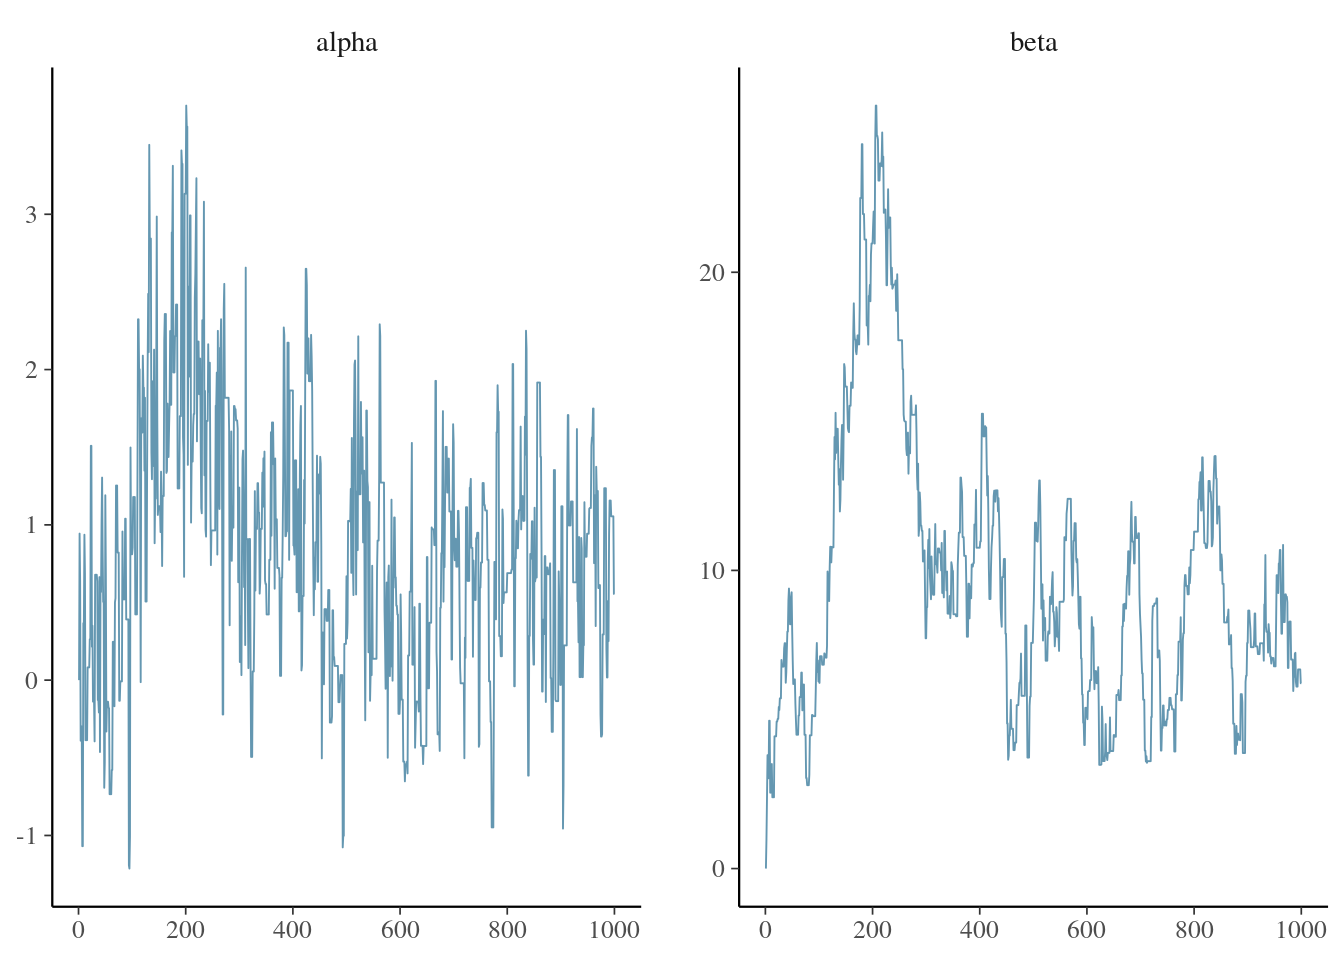
\includegraphics[width=8cm]{unnamed-chunk-7-1.png}}
  %    \only<4>{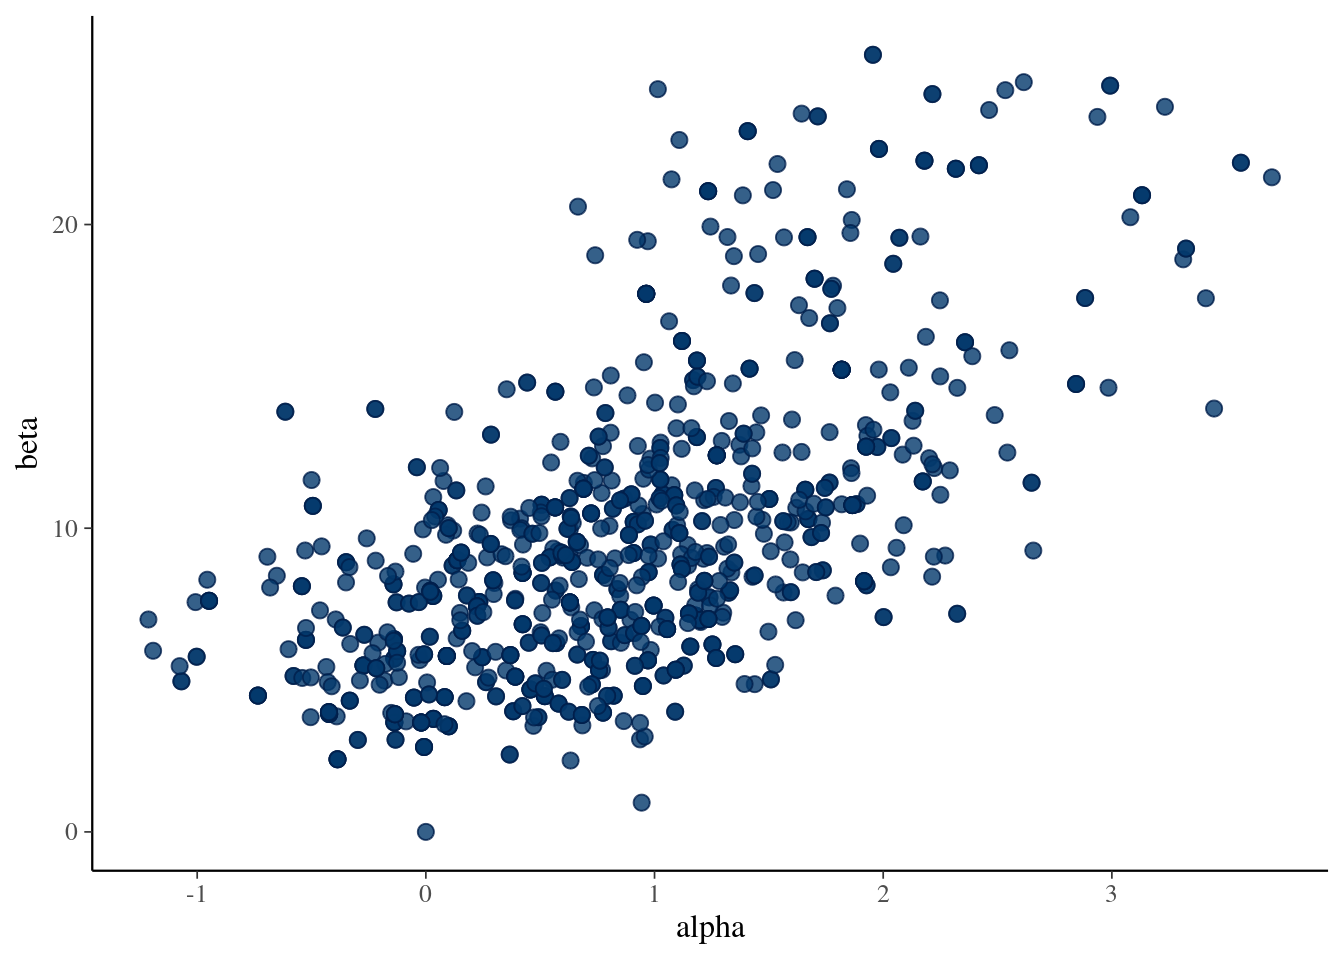
\includegraphics[width=8cm]{unnamed-chunk-9-1.png}}
  %    \only<5>{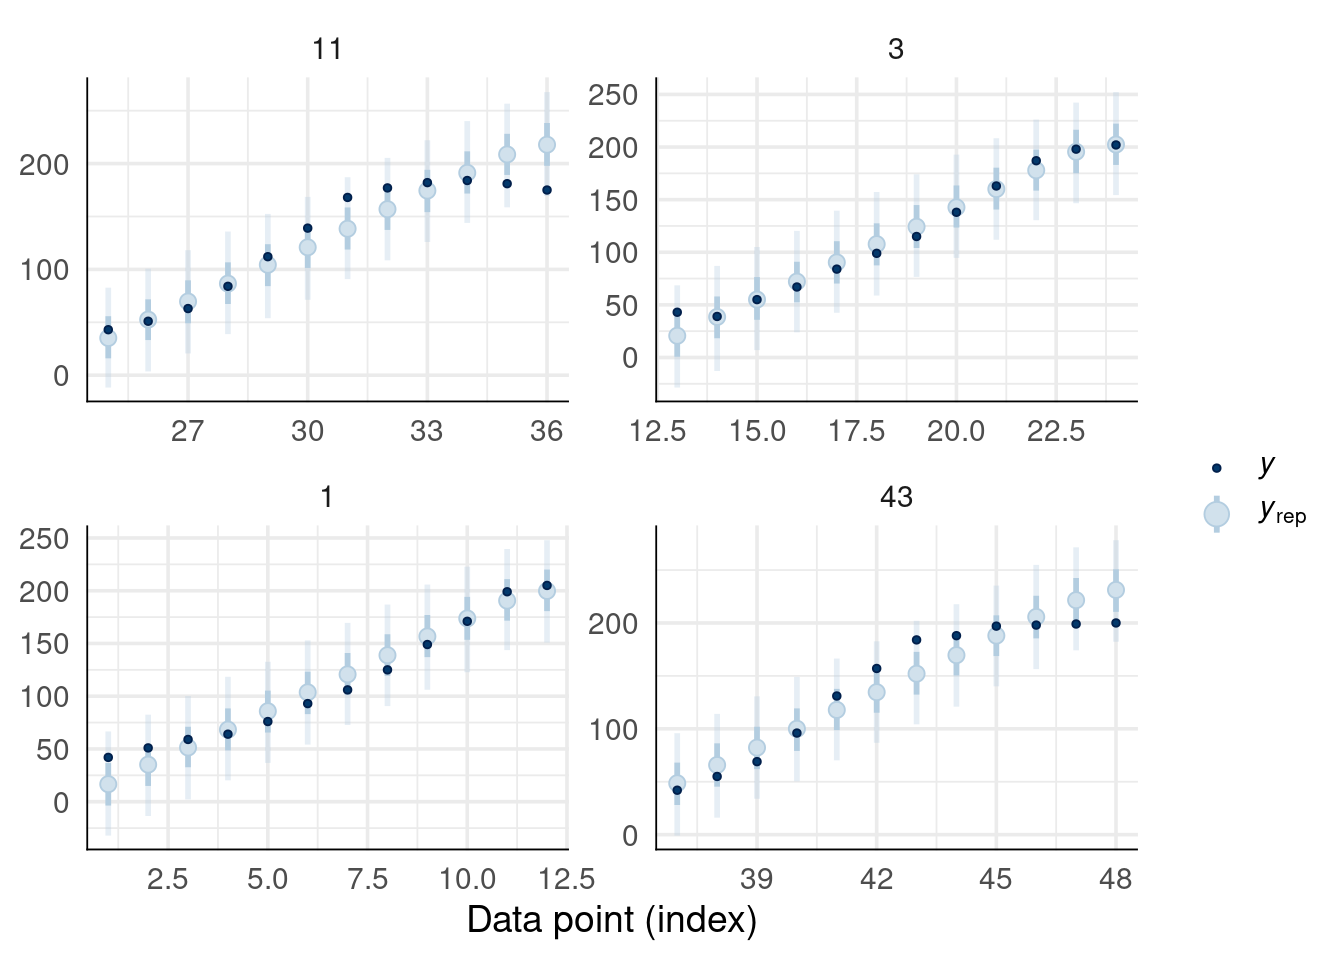
\includegraphics[width=8cm]{unnamed-chunk-12-1.png}}
  %    \only<6>{\includegraphics[width=8cm]{unnamed-chunk-13-1.png}}
  %    \only<7>{\includegraphics[width=8cm]{unnamed-chunk-15-1.png}}
  %    \only<8>{\includegraphics[width=8cm]{unnamed-chunk-21-1.png}}
  %    \only<9>{\includegraphics[width=8cm]{unnamed-chunk-31-1.png}}
  %  \end{itemize}
    \vspace{0.25\baselineskip}
    \item<2-> Demo \url{https://chi-feng.github.io/mcmc-demo/}
    \end{itemize}
  \end{frame}


  % \item Different parameterizations matter

\begin{frame}{Divergences}

  \begin{itemize}
  \item HMC specific: indicates that Hamiltonian dynamic simulation
    has problems with unexpected fast changes in log-density
    \begin{itemize}
    \item indicates possibility of biased estimates
    \end{itemize}
  \item {\small \url{http://mc-stan.org/users/documentation/case-studies/divergences_and_bias.html}}
     \only<1>{\phantom{\includegraphics[width=8cm]{unnamed-chunk-6-1.png}}}
     \only<2>{\includegraphics[width=8cm]{unnamed-chunk-6-1.png}}
     \only<3>{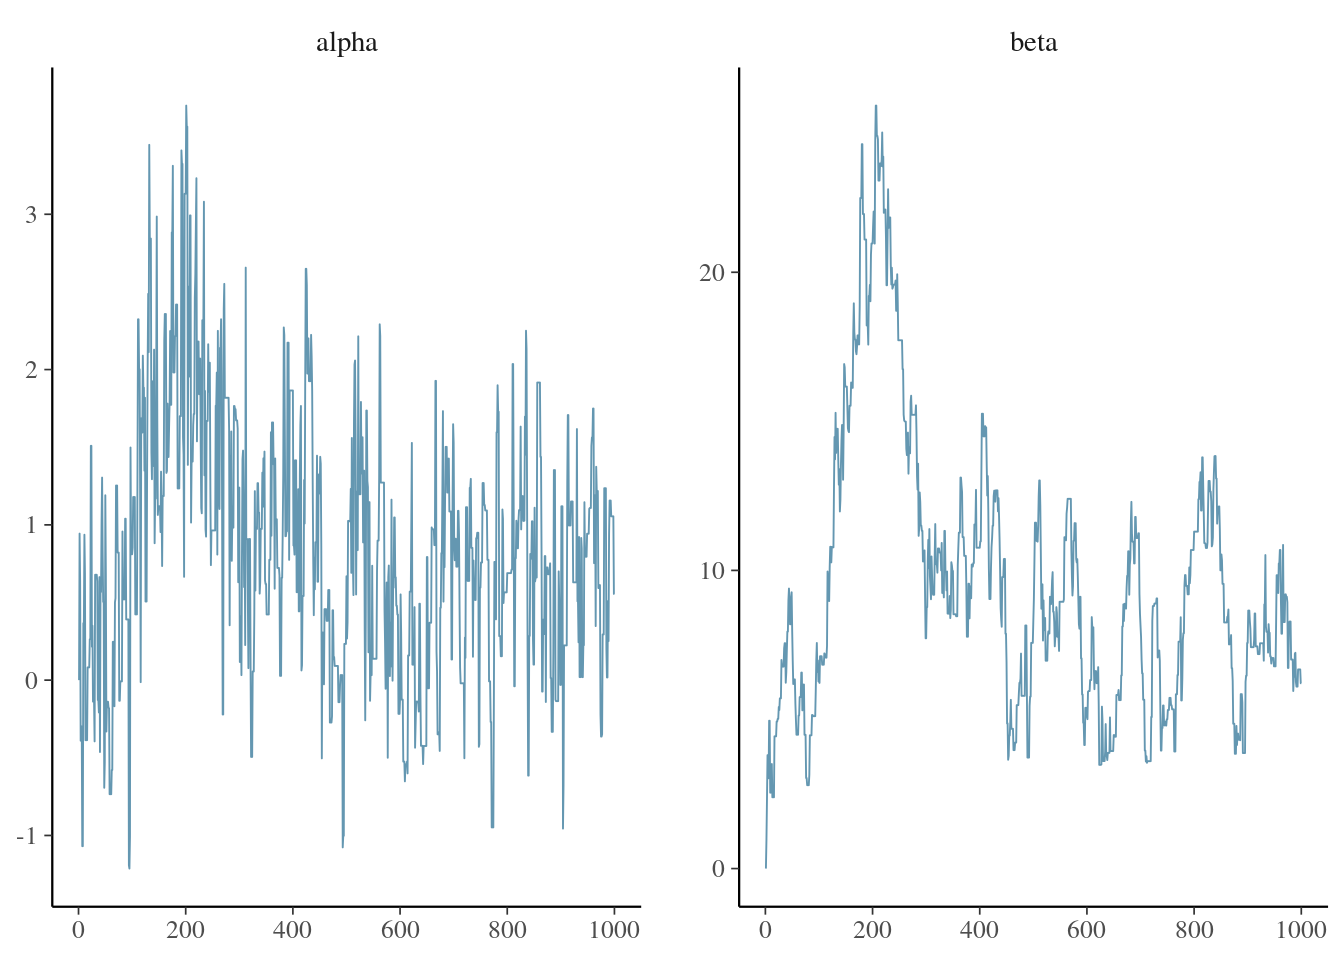
\includegraphics[width=8cm]{unnamed-chunk-7-1.png}}
     \only<4>{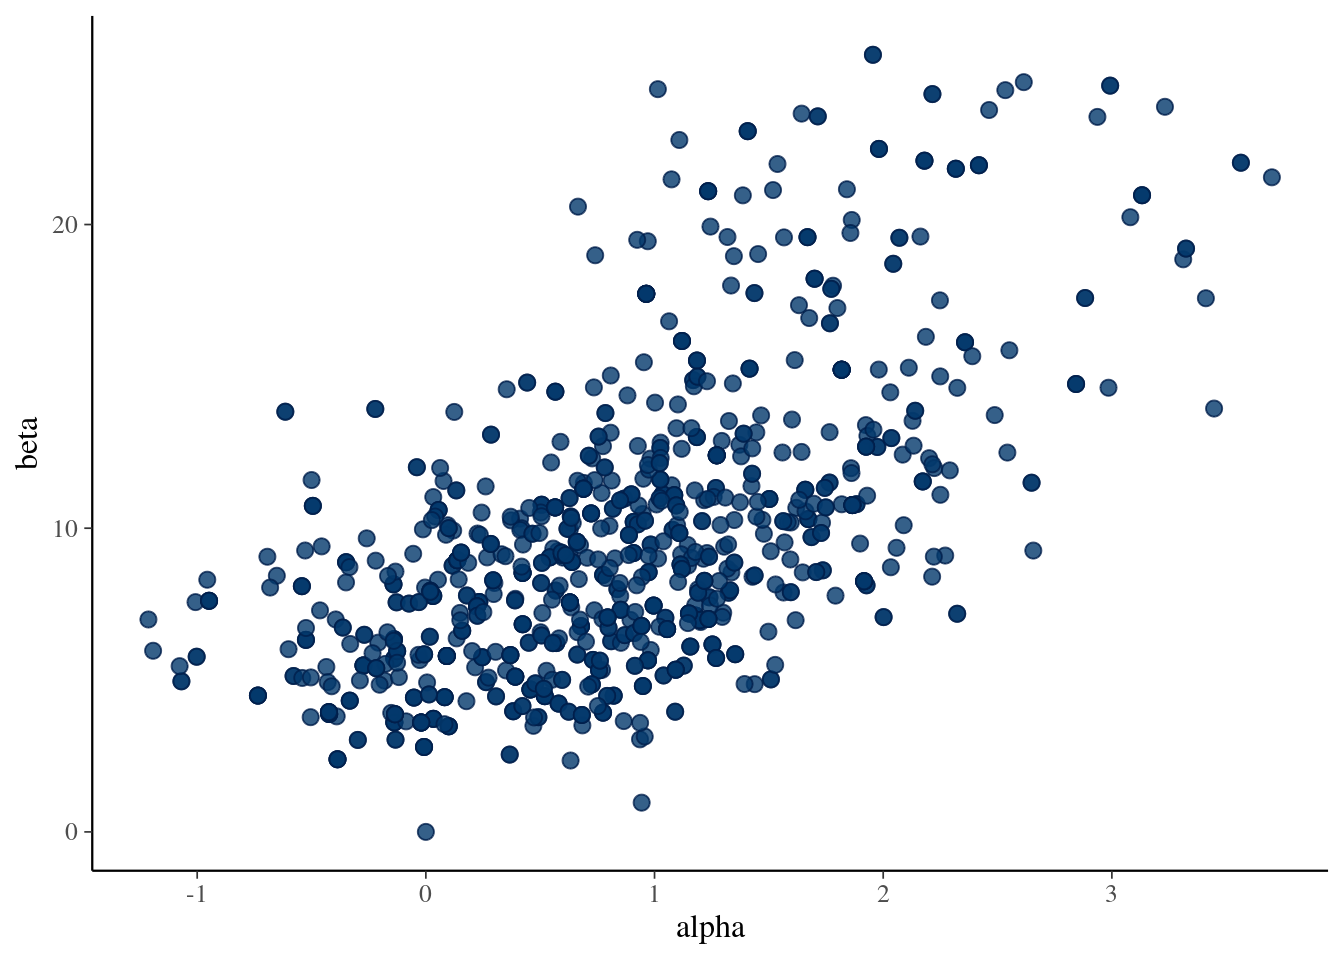
\includegraphics[width=8cm]{unnamed-chunk-9-1.png}}
     \only<5>{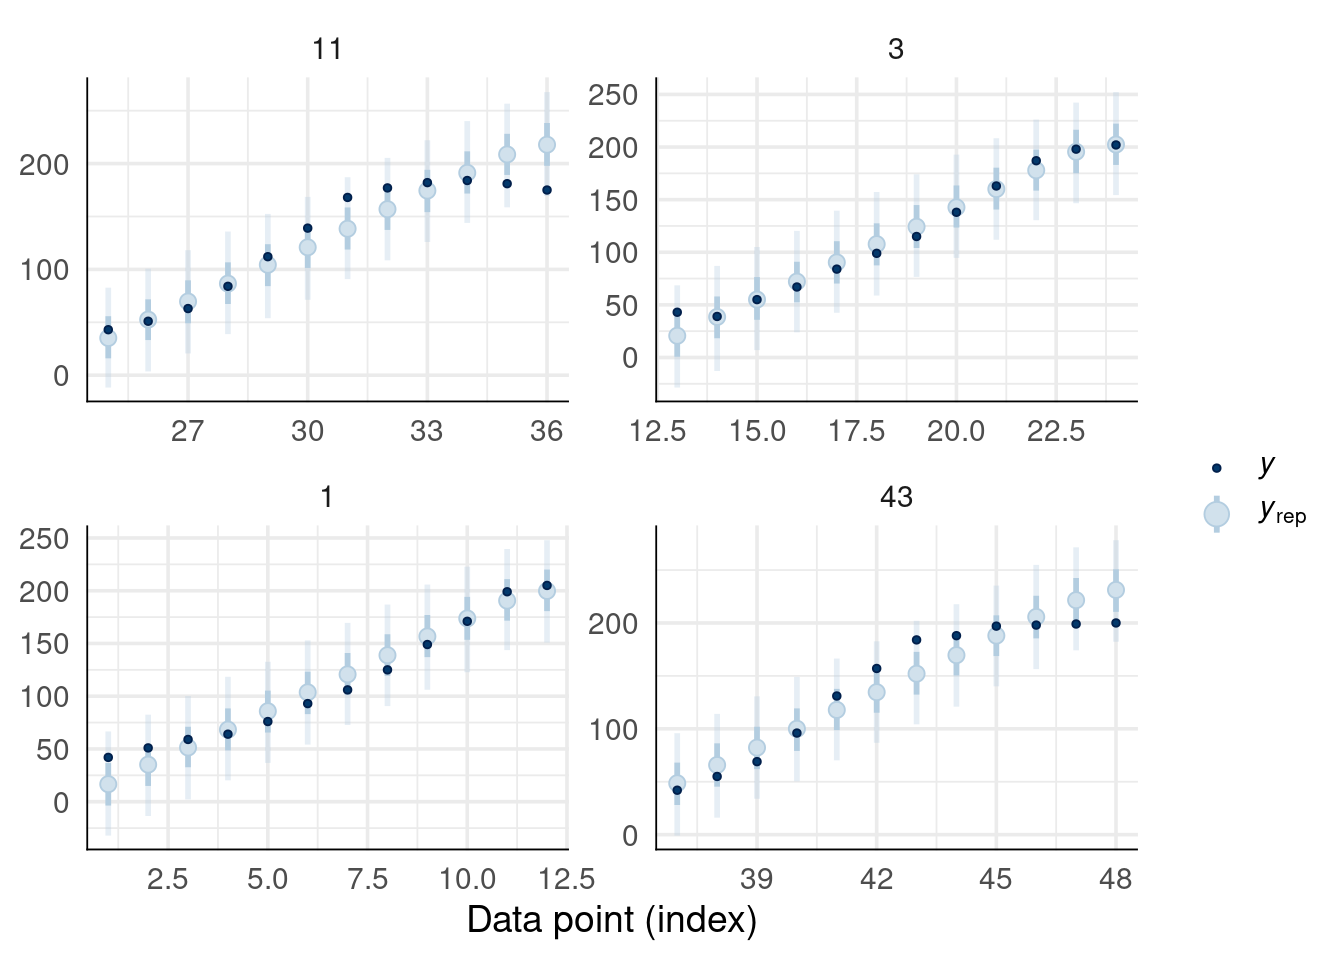
\includegraphics[width=8cm]{unnamed-chunk-12-1.png}}
     \only<6>{\includegraphics[width=8cm]{unnamed-chunk-13-1.png}}
     \only<7>{\includegraphics[width=8cm]{unnamed-chunk-15-1.png}}
     \only<8>{\includegraphics[width=8cm]{unnamed-chunk-21-1.png}}
     \only<9>{\includegraphics[width=8cm]{unnamed-chunk-31-1.png}}
  \end{itemize}
\end{frame}


\begin{frame}{Problematic distributions}

  \begin{itemize}
  \item<1-> Nonlinear dependencies
    \begin{itemize}
    \item simple mass matrix scaling doesn't help
    \end{itemize}
  \item<2-> Funnels
    \begin{itemize}
    \item optimal step size depends on location
    \end{itemize}
  \item<3-> Multimodal
    \begin{itemize}
    \item difficult to move from one mode to another
    \end{itemize}
  \item<4-> Long-tailed with non-finite variance and mean
    \begin{itemize}
    \item efficiency of exploration is reduced
    \item central limit theorem doesn't hold for mean and variance
    \end{itemize}
  \end{itemize}

\end{frame}

\begin{frame}{Some other recent HMC and gradient based variants}

  \begin{itemize}
  \item ChEES-HMC (Hoffman et al., 2021)
    \begin{itemize}
    \item a GPU friendly adapted but fixed simulation length
    \item static after adaptation
    \end{itemize}
  \item MEADS (Hoffman \& Sountsov, 2022)
    \begin{itemize}
    \item a GPU friendly multi-chain adaptation for generalized HMC (Horowitz, 1991) in
      which the momentum is partially updated frequently
    \item instead of simulation length, need to choose the partial
      update rate
    \end{itemize}
  \item MALT (Riou-Durand and Vogrinc, 2022; Riou-Durand et al., 2022)
    \begin{itemize}
    \item a GPU friendly method related to GHMC
    \item but avoids momentum flips after rejection
    \end{itemize}
  % \item Apogee to Apogee Path Sampler (AAPS, Sherlock et al., 2021)
  %   \begin{itemize}
  %   \item a dynamic HMC
  %   \end{itemize}
  \end{itemize}
  
\end{frame}

\begin{frame}{Probabilistic programming language}
  
  \begin{itemize}
  \item Wikipedia ``A probabilistic programming language (PPL) is a
    programming language designed to describe probabilistic models
    and then perform inference in those models''
    \pause
  \item To make probabilistic programming useful
    \begin{itemize}
    \item inference has to be as automatic as possible
    \item diagnostics for telling if the automatic inference doesn't work
    \item easy workflow (to reduce manual work)
    \item fast enough (manual work replaced with automation)
    \end{itemize}
  \end{itemize}
\end{frame}

\begin{frame}{Probabilistic programming}
  
  \begin{itemize}
  \item Enables agile workflow for developing probabilistic models
    \begin{itemize}
    \item language
    \item automated inference
    \item diagnostics
    \end{itemize}
  \item Many frameworks
    Stan, PyMC, Pyro (Uber), TFP (Google), Turing.jl, JAGS, ELFI, ...
    \begin{itemize}
    \item Short review of the landscape:\\
      {\small Štrumbelj et al. (2023). Past, Present, and Future of
        Software for Bayesian Inference. \textit{Statistical Science},
        accepted for publication. Preprint
        \url{http://www.stat.columbia.edu/~gelman/research/published/Bayesian_software_review-8.pdf}}.
      
    \end{itemize}
  \end{itemize}
  
\end{frame}

\begin{frame}{Stan - probabilistic programming framework}

   \begin{itemize}
   \item Language, inference engine, user interfaces, documentation,
     case studies, diagnostics, packages, ...
     \begin{itemize}
     \item autodiff to compute gradients of the log density
     \end{itemize}
   \item<2-> Most popular, with more than 200K users in social, biological, and
     physical sciences, medicine, engineering, and business
     
   \item<3-> Several full time developers, 40+ developers, more than 100 contributors
   \item<4-> R, Python, Julia, Scala, Stata, command line interfaces
    \item<4-> More than 200 R packages using Stan
   \end{itemize}
  \vfill
  \begin{center}
    \includegraphics[width=1.5cm]{Stan_blue.png}\\
    \url{mc-stan.org}
  \end{center}
\end{frame}

\begin{frame}{Stan}

  \begin{itemize}
  \item Stanislaw Ulam (1909-1984)
    \begin{itemize}
    \item Monte Carlo method
    \item H-Bomb
    \end{itemize}
  \end{itemize}
  
\end{frame}

\begin{frame}[fragile]{Binomial model - Stan code}

  {Domain-specific language} for constructing models


\small
\setminted{gray}  

{\only<1>{\setminted{gray=false}}
\begin{minted}{stan}
data {
  int<lower=0> N;         // number of experiments
  int<lower=0,upper=N> y; // number of successes
}
\end{minted}
}

{\only<2>{\setminted{gray=false}}
\begin{minted}{stan}
parameters {
  real<lower=0,upper=1> theta; // parameter of the binomial
}
\end{minted}
}
  
{\only<3>{\setminted{gray=false}}
\begin{minted}{stan}
model {
  theta ~ beta(1, 1);      // prior
  y ~ binomial(N, theta);  // observation / data model
}
\end{minted}
}

\end{frame} 


\begin{frame}[fragile]{Binomial model - Stan code}
  
  {\small
  \begin{minted}{stan}
data {
  int<lower=0> N;         // number of experiments
  int<lower=0,upper=N> y; // number of successes
}
\end{minted}
  }

  \begin{itemize}
  \item Data type and size are declared
  \item Stan checks that given data matches type and constraints
    \begin{itemize}
    \item<2-> If you are not used to strong typing, this may
      feel annoying, but it will reduce the probability of coding
      errors, which will reduce probability of data analysis errors
    \end{itemize}
  \end{itemize}
\end{frame}

\begin{frame}[fragile]{Binomial model - Stan code}

  {\small
\begin{minted}{stan}
parameters {
  real<lower=0,upper=1> theta; // parameter of the binomial
}
\end{minted}
  }

  \begin{itemize}
  \item Only continuous parameters allowed (discrete parameters can
    often be integerated out in the model block)
  \item Parameters may have constraints
  \item Stan makes transformation to unconstrained space and samples in unconstrained space
    \begin{itemize}
    \item e.g. log transformation for <lower=a> 
    \item e.g. logit transformation for <lower=a,upper=b> 
    \end{itemize}
  \item<2-> For these declared transformation Stan automatically takes
    into account the Jacobian of the transformation (see BDA3 p. 21)
  \end{itemize}
\end{frame}

\begin{frame}[fragile]{Binomial model - Stan code}

  \vspace{-\baselineskip}
  {\small
\begin{minted}{stan}
model {
  theta ~ beta(1, 1);     // prior
  y ~ binomial(N, theta); // observation model
}
\end{minted}
  }

    \vspace{-0.5\baselineskip}
    \begin{itemize}
    \item $\sim$ defines a \textit{distribution statement}
      \begin{itemize}
      \item[] e.g. \textit{y is distributed as binomial(N, theta)}
      \end{itemize}
    \item<2-> these can be written also as \textit{log density increment statements}
      \begin{itemize}
      \item[] left side of $|$ denotes what is distributed as, e.g., binomial
      \end{itemize}
    \end{itemize}

    \pause
    \vspace{-0.5\baselineskip}
  {\small
\begin{minted}{stan}
model {
  target += beta_lpdf(theta | 1, 1);
  target += binomial_lpmf(y | N, theta);
}
\end{minted}
  }

    \vspace{-0.5\baselineskip}
    \begin{itemize}
    \item<3-> {\tt target} is the log posterior density (Lecture 4 discussed log)
    \item<4-> {\tt \_lpdf} for continuous, {\tt \_lpmf} for discrete distributions (left of {\tt |})
    \item<5-> if \texttt{y} are data, and \texttt{theta} is a parameter, then that term defines log likelihood
    \item<6-> for Stan sampler there is no difference between prior and likelihood, all that matters is the final {\tt target}
    \end{itemize}

\end{frame} 

% \begin{frame}[fragile]

%   {\Large\color{navyblue} Binomial model - Stan code}
  
%   {\small
% \begin{minted}{stan}
% model {
%   theta ~ beta(1,1);     //prior
%   y ~ binomial(N,theta); // observation model
% }
% \end{minted}
%  }

%     \begin{itemize}
%     \item $\sim$ is syntactic sugar and this could be also written as
%     \end{itemize}

%   {\small
% \begin{minted}{stan}
% model {
%   target +=  beta_lpdf(theta | 1, 1);
%   target +=  binomial_lpmf(y | N, theta);
% }
% \end{minted}
%  }

%     \begin{itemize}
%     \end{itemize}
    
% \end{frame}

\begin{frame}{Stan}
  
  \begin{itemize}
  \item You can write in Stan language any program to compute the
    log density (Stan language is Turing complete)
  \item<2-> Stan compiles (transplies) the model written in Stan language to C++
    \begin{itemize}
    \item this makes the sampling for complex models and bigger data faster
    \item also makes Stan models easily portable, you can use your own
      favorite interface and scripting language for manipulating data
      and inference results (e.g. R, Python, Julia, Stata, ...)
    \end{itemize}
  \end{itemize}

\end{frame}

\begin{frame}[fragile]{CmdStanR}

  {\small
    \setminted{gray}
    {\only<1>{\setminted{gray=false}}
      RStan
\begin{minted}{r}
library(cmdstanr) 
options(mc.cores = 1)
\end{minted}
    }
{\only<2>{\setminted{gray=false}}
\begin{minted}{r}
d_bin <- list(N = 10, y = 7)
mod_bin <- cmdstan_model(stan_file = 'binom.stan')
fit_bin <- mod_bin$sample(data = d_bin)
\end{minted}
}
}
\end{frame}

\begin{frame}[fragile]{PyStan}

  {\small
    \setminted{gray}
    {\only<1>{\setminted{gray=false}}
      PyStan
\begin{minted}{py}
import pystan
import stan_utility
\end{minted}
    }
    {\only<2>{\setminted{gray=false}}
\begin{minted}{py}
data = dict(N=10, y=8)
model = stan_utility.compile_model('binom.stan')
fit = model.sampling(data=data)
\end{minted}
    }
  }
\end{frame}

\begin{frame}{Stan}
  
  \begin{itemize}
  \item Compilation (unless previously compiled model available)
  \item Warm-up including adaptation
  \item Sampling
  \item Generated quantities
  \item Save posterior draws
  \item Report divergences, ESS, $\widehat{R}$
  \end{itemize}

\end{frame}

\begin{frame}{Difference between proportions}
  
\begin{itemize}
  \item An experiment was performed to estimate the effect of
    beta-blockers on mortality of cardiac patients
  \item A group of
    patients were randomly assigned to treatment and control groups:
    \begin{itemize}
    \item out of 674 patients receiving the control, 39 died
    \item out of 680 receiving the treatment, 22 died
    \end{itemize}
  \end{itemize}
\end{frame}

\begin{frame}[fragile]{Difference between proportions}

%  Beta-blockers $N_1 = 674, y_1 = 39, N_2 = 680, y_2 = 22$
  
  \vspace{-0.5\baselineskip}
  {\small
    \setminted{gray}
    {\only<1>{\setminted{gray=false}}
\begin{minted}{stan}
data {
  int<lower=0> N1;
  int<lower=0> y1;
  int<lower=0> N2;
  int<lower=0> y2;
}
\end{minted}
    }
    \vspace{-1.5\baselineskip}
    {\only<2>{\setminted{gray=false}}
\begin{minted}{stan}
parameters {
  real<lower=0,upper=1> theta1;
  real<lower=0,upper=1> theta2;
}
\end{minted}
    }
    \vspace{-1.5\baselineskip}
    {\only<3>{\setminted{gray=false}}
\begin{minted}{stan}
model {
  theta1 ~ beta(1, 1);
  theta2 ~ beta(1, 1);
  y1 ~ binomial(N1, theta1);
  y2 ~ binomial(N2, theta2);
}
\end{minted}
    }
    \vspace{-1.5\baselineskip}
    {\only<4>{\setminted{gray=false}}
\begin{minted}{stan}
generated quantities {
  real oddsratio;
  oddsratio = (theta2/(1-theta2))/(theta1/(1-theta1));
}
\end{minted}
    }
  }
\end{frame}

\begin{frame}[fragile]{Difference between proportions}

%  Beta-blockers $N_1 = 674, y_1 = 39, N_2 = 680, y_2 = 22$
  
  {\small
\begin{minted}{stan}
generated quantities {
  real oddsratio;
  oddsratio = (theta2/(1-theta2))/(theta1/(1-theta1));
}
\end{minted}
    }

    \begin{itemize}
    \item generated quantities is run after the sampling
    \end{itemize}
    
\end{frame}

\begin{frame}[fragile]{Difference between proportions}
  
  {\small
\begin{minted}{r}
d_bin2 <- list(N1 = 674, y1 = 39, N2 = 680, y2 = 22)
mod_bin2 <- cmdstan_model(stan_file = 'binom2.stan')
fit_bin2 <- mod_bin2$sample(data = d_bin2, refresh=1000)
\end{minted}
  }

  {\footnotesize
\begin{minted}{text}
> Running MCMC with 4 parallel chains...

Chain 1 Iteration:    1 / 2000 [  0%]  (Warmup) 
Chain 1 Iteration: 1000 / 2000 [ 50%]  (Warmup) 
Chain 1 Iteration: 1001 / 2000 [ 50%]  (Sampling) 
Chain 1 Iteration: 2000 / 2000 [100%]  (Sampling) 
...
All 4 chains finished successfully.
Mean chain execution time: 0.0 seconds.
Total execution time: 0.2 seconds.
\end{minted}
  }

\end{frame}

\begin{frame}[fragile]{Difference between proportions}
  
  {\small
\begin{minted}{r}
options(posterior.num_args=list(sigfig=2))
fit_bin2$summary()
\end{minted}
  }

  {\scriptsize
\begin{minted}{text}
  variable    mean  median     sd    mad      q5     q95  rhat ess_bulk ess_tail
1 lp__     -2.5e+2 -2.5e+2 1.0    0.74   -2.6e+2 -2.5e+2   1.0    1751.    2231.
2 theta1    5.9e-2  5.9e-2 0.0093 0.0093  4.5e-2  7.5e-2   1.0    3189.    2657.
3 theta2    3.4e-2  3.3e-2 0.0069 0.0067  2.3e-2  4.6e-2   1.0    3229.    2163.
4 oddsratio 5.7e-1  5.5e-1 0.16   0.15    3.5e-1  8.7e-1   1.0    2998.    2685.
\end{minted}
  }

  \begin{itemize}
  \item<2-> {\tt lp\_\_} is the log density, ie, same as {\tt target}
  \end{itemize}

\end{frame}

\begin{frame}[fragile]{HMC specific diagnostics}
  
  {\small
\begin{minted}{r}
fit_bin2$diagnostic_summary(diagnostics = c("divergences",
                                            "treedepth"))
\end{minted}
  }

  {\footnotesize
\begin{minted}{text}
$num_divergent
[1] 0 0 0 0

$num_max_treedepth
[1] 0 0 0 0
\end{minted}
  }

\end{frame}

\begin{frame}[fragile]{Difference between proportions (bayesplot)}
  
  {\small
\begin{minted}{r}
draws <- fit_bin2$draws(format = "df")
mcmc_hist(draws, pars = 'oddsratio') +
  geom_vline(xintercept = 1) +
  scale_x_continuous(breaks = c(seq(0.25,1.5,by=0.25)))
\end{minted}
  }

  \begin{center}
  \includegraphics[width=9cm]{betablockoddsratio.pdf}
\end{center}
\end{frame}

\begin{frame}[fragile]{Difference between proportions (ggplot2)}

  \vspace{-0.5\baselineskip}
  {\small
\begin{minted}{r}
draws <- fit_bin2$draws(format = "df")
draws |> ggplot(aes(x=oddsratio)) +
  geom_histogram() +
  geom_vline(xintercept = 1) +
  scale_x_continuous(breaks = c(seq(0.25,1.5,by=0.25)))
\end{minted}
  }

  \begin{center}
  \includegraphics[width=9cm]{betablockoddsratio_ggplot.pdf}
\end{center}
\end{frame}

\begin{frame}[fragile]{Difference between proportions (ggdist dot plot)}
  
  \vspace{-0.5\baselineskip}
  {\small
\begin{minted}{r}
draws <- fit_bin2$draws(format = "df")
draws |> ggplot(aes(x=oddsratio)) +
  geom_dotsinterval() +
  geom_vline(xintercept = 1) +
  scale_x_continuous(breaks = c(seq(0.25,1.5,by=0.25)))
\end{minted}
  }

  \begin{center}
  \includegraphics[width=9cm]{betablockoddsratio_dots.pdf}
\end{center}
\end{frame}

\begin{frame}[fragile]{Difference between proportions (probability and MCSE)}

  Probability (and corresponding MCSE) that oddsratio<1
  \\~
  
{\small
\begin{minted}{r}
> draws |>
    mutate_variables(p_oddsratio_lt_1 =
                     as.numeric(oddsratio<1)) |>
    subset_draws("p_oddsratio_lt_1") |>
    summarise_draws(prob=mean, MCSE=mcse_mean)
\end{minted}
\begin{minted}{text}
  variable            prob    MCSE
  p_oddsratio_lt_1    0.99  0.0023
\end{minted}
  }

\end{frame}

\begin{frame}[fragile]{posterior object formats}

  \vspace{-.5\baselineskip}
  Default is \texttt{draws\_array}
  
{\footnotesize
\begin{minted}{r}
> fit_bin2$draws()
\end{minted}
  \vspace{-\baselineskip}
\begin{minted}[highlightlines={1}]{text}
# A draws_array: 1000 iterations, 4 chains, and 4 variables
, , variable = lp__

         chain
iteration    1    2    3    4
        1 -253 -253 -254 -253
        2 -253 -253 -255 -252
        3 -254 -252 -254 -253
        4 -255 -253 -254 -254
        5 -253 -253 -253 -253

, , variable = theta1

         chain
iteration     1     2     3     4
        1 0.054 0.052 0.045 0.049
        2 0.062 0.060 0.070 0.058
...
\end{minted}
  }

\end{frame}

\begin{frame}[fragile]{posterior object formats}

  \texttt{draws\_df} looks prettier and works with \texttt{ggplot()}
  
  {\footnotesize
\begin{minted}{r}
> fit_bin2$draws(format ="df")
\end{minted}
  \vspace{-\baselineskip}
\begin{minted}[highlightlines={1}]{text}
# A draws_df: 1000 iterations, 4 chains, and 4 variables
   lp__ theta1 theta2 oddsratio
1  -253  0.054  0.033      0.59
2  -253  0.062  0.035      0.55
3  -254  0.047  0.026      0.54
4  -255  0.049  0.049      0.99
5  -253  0.068  0.035      0.50
6  -253  0.056  0.027      0.47
7  -253  0.071  0.031      0.43
8  -253  0.049  0.036      0.72
9  -253  0.049  0.036      0.72
10 -253  0.063  0.026      0.39
# ... with 3990 more draws
# ... hidden reserved variables {'.chain', '.iteration', '.draw'}
\end{minted}
  }

\end{frame}

\begin{frame}[fragile]{posterior object formats}

 \vspace{-0.8\baselineskip}
  \texttt{draws\_rvar} makes it easy to compute derived quantities
  
{\scriptsize
    \setminted{gray}
    {\only<1>{\setminted{gray=false}}
\begin{minted}{r}
> as_draws_rvars(fit_bin2$draws())
\end{minted}
  \vspace{-\baselineskip}
\begin{minted}[highlightlines={1}]{text}
# A draws_rvars: 1000 iterations, 4 chains, and 4 variables
$lp__: rvar<1000,4>[1] mean ± sd:
[1] -253 ± 1 

$theta1: rvar<1000,4>[1] mean ± sd:
[1] 0.059 ± 0.0093 

$theta2: rvar<1000,4>[1] mean ± sd:
[1] 0.034 ± 0.0069 

$oddsratio: rvar<1000,4>[1] mean ± sd:
[1] 0.57 ± 0.16
\end{minted}
  }
    \pause
    {\only<2>{\setminted{gray=false}}
\begin{minted}{r}
> with(draws, (theta2/(1-theta2))/(theta1/(1-theta1)))
\end{minted}
  \vspace{-\baselineskip}
\begin{minted}{text}
rvar<1000,4>[1] mean ± sd:
[1] 0.5689 ± 0.1577 
\end{minted}
      }
    \pause
    {\only<3>{\setminted{gray=false}}
\begin{minted}{r}
> draws$oddsratio<1
\end{minted}
  \vspace{-\baselineskip}
\begin{minted}{text}
rvar<1000,4>[1] mean ± sd:
[1] 0.9865 ± 0.1154 
\end{minted}
  }
}

\end{frame}

% \begin{frame}{Shinystan}

%   \begin{itemize}
%   \item Graphical user interface for analysing MCMC results
%   \end{itemize}
  
% \end{frame} 

\begin{frame}{Kilpisjärvi summer temperature}
  
  \begin{itemize}
  \item Temperature at Kilpisjärvi in June, July and August from 1952 to 2013
  \item Is there change in the temperature?
  \end{itemize}
  \begin{center}
    \includegraphics[width=10cm]{kilpis_data.pdf}
  \end{center}
  
\end{frame}

\begin{frame}[fragile]{Normal linear model}
  
  {\small
    \setminted{gray}
    {\only<1>{\setminted{gray=false}}
  \begin{minted}{stan}
data {
    int<lower=0> N;        // number of observations
    vector[N] x; 
    vector[N] y;  
}
\end{minted}
    }
    \vspace{-1.5\baselineskip}
    {\only<2>{\setminted{gray=false}}
\begin{minted}{stan}
parameters {
    real alpha;            // intercept
    real beta;             // slope
    real<lower=0> sigma;   // observation model sd
}
\end{minted}
    }
    \vspace{-1.5\baselineskip}
    {\only<3>{\setminted{gray=false}}
\begin{minted}{stan}
transformed parameters {
    vector[N] mu;
    mu = alpha + beta*x;  // linear model
}
\end{minted}
    }
    \vspace{-1.5\baselineskip}
    {\only<4>{\setminted{gray=false}}
\begin{minted}{stan}
model {
    y ~ normal(mu, sigma); // observation model
}
\end{minted}
    }
  }
  
\end{frame} 

\begin{frame}[fragile]{Normal linear model}
  
  {\small
  \begin{minted}{stan}
data {
    int<lower=0> N;        // number of observations
    vector[N] x; 
    vector[N] y;  
}
\end{minted}
  }

  \begin{itemize}
  \item difference between {\small\tt vector[N] x}\, and\, {\small\tt array[N] real x}
  \item<2-> only integer arrays: {\small\tt array[N] int x}
  \end{itemize}
  
\end{frame}

\begin{frame}[fragile]{Normal linear model}
  
  {\small
   { \setminted{gray}
  \begin{minted}{stan}
parameters {
    real alpha;            // intercept
    real beta;             // slope
    real<lower=0> sigma;   // observation model sd
}
\end{minted}
    }
    \vspace{-1.5\baselineskip}
\begin{minted}{stan}
transformed parameters {
    vector[N] mu;
    mu = alpha + beta*x;  // linear model
}
\end{minted}
  }
  
  \begin{itemize}
  \item transformed parameters are deterministic transformations of parameters and data
  \end{itemize}
\end{frame} 

\begin{frame}[fragile]{Student-$t$ linear model}
  
  {\small
  \begin{minted}[highlightlines={6,13,14}]{stan}
...
parameters {
  real alpha; 
  real beta; 
  real<lower=0> sigma;
  real<lower=1,upper=80> nu;
}
transformed parameters {
  vector[N] mu;
  mu = alpha + beta*x;
}
model {
  nu ~ gamma(2, 0.1);             // prior for nu
  y ~ student_t(nu, mu, sigma);  // observation model
}
  \end{minted}
}
\end{frame} 

\begin{frame}[fragile]{Priors for normal linear model}
  
  {\small
  \begin{minted}[highlightlines={5-8,16,17}]{stan}
data {
    int<lower=0> N; // number of observations 
    vector[N] x; // 
    vector[N] y; // 
    real pmualpha; // prior mean for alpha
    real psalpha;  // prior std for alpha
    real pmubeta;  // prior mean for beta
    real psbeta;   // prior std for beta
}
...
transformed parameters {
    vector[N] mu;
    mu = alpha + beta*x;
}
model {
    alpha ~ normal(pmualpha, psalpha); // prior for alpha
    beta ~ normal(pmubeta, psbeta);    // prior for beta
    y ~ normal(mu, sigma);             // observation model
}
  \end{minted}
}
\end{frame} 

\begin{frame}{Priors}

  \begin{itemize}
  \item Prior for temperature increase?
  \end{itemize}

\end{frame}

\begin{frame}{Kilpisjärvi summer temperature}

  Posterior fit
  
  \begin{center}
    \includegraphics[width=10cm]{kilpis_lin_pfit.pdf}
  \end{center}

\end{frame}

\begin{frame}{Kilpisjärvi summer temperature}

  Posterior draws of alpha and beta
  
  \begin{center}
    \includegraphics[width=10cm]{kilpis_lin_mcmc_scatter.pdf}
  \end{center}
 
\end{frame}

\begin{frame}[fragile]{Kilpisjärvi summer temperature}
  
  Posterior draws of alpha and beta
  
  \begin{center}
    \includegraphics[width=10cm]{kilpis_lin_mcmc_scatter.pdf}
  \end{center}

{\scriptsize
\begin{minted}{r}
Warning: 1 of 4000 (0.0%) transitions hit the maximum treedepth limit of 10.
See https://mc-stan.org/misc/warnings for details.
\end{minted}
}
  
\end{frame}

\begin{frame}[fragile]{Linear regression model in Stan}

Center the data inside the model code
  
{\footnotesize
\begin{minted}[gray]{stan}
data {
  int<lower=0> N; // number of observations
  vector[N] x; 
  vector[N] y; 
  real xpred;     // covarite values for prediction
}
\end{minted}
\begin{minted}{stan}
transformed data {
  vector[N] x_std;
  vector[N] y_std;
  real xpred_std;
  x_std = (x - mean(x)) / sd(x);
  y_std = (y - mean(y)) / sd(y);
  xpred_std = (xpred - mean(x)) / sd(x);
}
\end{minted}
}
\end{frame}

\begin{frame}[fragile]{Kilpisjärvi summer temperature}
  
  Posterior draws of alpha and beta when data is centered
  
  \begin{center}
    \includegraphics[width=10cm]{kilpis_lin_std_mcmc_scatter.pdf}
  \end{center}

\end{frame}

\begin{frame}[fragile]{Kilpisjärvi summer temperature}

Without centering  
{\footnotesize
\begin{minted}{r}
> fit_lin$summary(variables=c("alpha","beta"),
                  default_convergence_measures())
\end{minted}
  \vspace{-\baselineskip}
\begin{minted}{text}
  variable    rhat ess_bulk ess_tail
  alpha        1.0     919.     897.
  beta         1.0     919.     895.
\end{minted}
  }

With centering  
{\footnotesize
\begin{minted}{r}
> fit_lin_std$summary(variables=c("alpha","beta"),
                      default_convergence_measures())
\end{minted}
  \vspace{-\baselineskip}
\begin{minted}{text}
  variable    rhat ess_bulk ess_tail
  alpha        1.0    3872.    2616.
  beta         1.0    3770.    2396.
\end{minted}
  }
\end{frame}

\begin{frame}[fragile]{RStanARM}

  \begin{itemize}
  \item \texttt{RStanARM} provides simplified model description with
    pre-compiled models
    \begin{itemize}
    \item no need to wait for compilation
    \item a restricted set of models
    \end{itemize}
  \end{itemize}

Two group Binomial model:
  {\footnotesize
\begin{minted}{r}
d_bin2 <- data.frame(N = c(674, 680), y = c(39,22), grp2 = c(0,1))
fit_bin2 <- stan_glm(y/N ~ grp2, family = binomial(), data = d_bin2,
                    weights = N)
\end{minted}
  }
% \begin{minted}{r}
% draws_bin2 <- as.data.frame(fit_bin2) %>%
%   mutate(theta1 = plogis(`(Intercept)`),
%          theta2 = plogis(`(Intercept)` + grp2),
%          oddsratio = (theta2/(1-theta2))/(theta1/(1-theta1)))

% mcmc_hist(draws_bin2, pars='oddsratio')
% \end{minted}
%     }
    
\end{frame} 


\begin{frame}[fragile]{RStanARM}

  \begin{itemize}
  \item \texttt{RStanARM} provides simplified model description with
    pre-compiled models
    \begin{itemize}
    \item no need to wait for compilation
    \item a restricted set of models
    \end{itemize}
  \end{itemize}

Two group Binomial model:
  {\footnotesize
\begin{minted}{r}
d_bin2 <- data.frame(N = c(674, 680), y = c(39,22), grp2 = c(0,1))
fit_bin2 <- stan_glm(y/N ~ grp2, family = binomial(), data = d_bin2,
                    weights = N)
\end{minted}
  }
    Normal linear model
  {\footnotesize
\begin{minted}{r}
    fit_lin <- stan_glm(temp ~ year, data = d_lin)
\end{minted}
  }
% \begin{minted}{r}
% draws_bin2 <- as.data.frame(fit_bin2) %>%
%   mutate(theta1 = plogis(`(Intercept)`),
%          theta2 = plogis(`(Intercept)` + grp2),
%          oddsratio = (theta2/(1-theta2))/(theta1/(1-theta1)))

% mcmc_hist(draws_bin2, pars='oddsratio')
% \end{minted}
%     }
    
\end{frame} 


\begin{frame}[fragile]{brms}

  \begin{itemize}
  \item \texttt{brms} provides simplified model description
    \begin{itemize}
    \item[+] a larger set of models than \texttt{RStanARM}, but still restricted
    \item[-] need to wait for the compilation
    \end{itemize}
  \end{itemize}

  {\footnotesize
\begin{minted}{r}
fit_bin2 <- brm(y | trials(N) ~ grp2, family = binomial(), data = d_bin2)


fit_lin_t <- brm(temp ~ year, data = d_lin, family = student())
\end{minted}
  }
    
\end{frame} 

\begin{frame}{Extreme value analysis}

Geomagnetic storms

\includegraphics[width=12cm]{stan_gpareto_geomev.png}  

\end{frame}

\begin{frame}[fragile]{Extreme value analysis}
  
  {\footnotesize
    \setminted{gray}
    {\only<1>{\setminted{gray=false}}
  \begin{minted}{stan}
data {
  int<lower=0> N;
  vector<lower=0>[N] y;
  int<lower=0> Nt;
  vector<lower=0>[Nt] yt;
}
\end{minted}
    }
    \vspace{-1.5\baselineskip}
    {\only<2>{\setminted{gray=false}}
\begin{minted}{stan}
transformed data {
  real ymax = max(y);
}
parameters {
  real<lower=0> sigma; 
  real<lower=-sigma/ymax> k; 
}
\end{minted}
    }
    \vspace{-1.5\baselineskip}
    {\only<3>{\setminted{gray=false}}
\begin{minted}{stan}
model {
  y ~ gpareto(k, sigma);
}
\end{minted}
    }
    \vspace{-1.5\baselineskip}
    {\only<4>{\setminted{gray=false}}
\begin{minted}{stan}
generated quantities {
  vector[Nt] predccdf = gpareto_ccdf(yt, k, sigma);
}
  \end{minted}
  }
}  
\end{frame} 

\begin{frame}[fragile]{User defined functions}
  
  \vspace{-.75\baselineskip}
  {\footnotesize
    \setminted{gray}
    {\only<1>{\setminted{gray=false}}
  \begin{minted}{stan}
functions {
  real gpareto_lpdf(vector y, real k, real sigma) {
    // generalised Pareto log pdf with mu=0
    // should check and give error if k<0 
    // and max(y)/sigma > -1/k
    int N;
    N <- dims(y)[1];
    if (abs(k) > 1e-15)
      return -(1+1/k)*sum(log1pv(y*k/sigma)) -N*log(sigma);
    else
      return -sum(y/sigma) -N*log(sigma); // limit k->0
  }
\end{minted}
    }
    \vspace{-1.25\baselineskip}
    {\only<2>{\setminted{gray=false}}
\begin{minted}{stan}
  vector gpareto_ccdf(vector y, real k, real sigma) {
    // generalised Pareto log ccdf with mu=0
    // should check and give error if k<0 
    // and max(y)/sigma < -1/k
    if (abs(k) > 1e-15)
      return exp((-1/k)*log1pv(y/sigma*k));
    else
      return exp(-y/sigma); // limit k->0
  }
}
  \end{minted}
    }
    }
\end{frame} 

\begin{frame}{Different interfaces}

  \begin{itemize}
  \item \texttt{CmdStanR} / \texttt{CmdStanPy}
    \begin{itemize}
    \item Interface on top of command-line program CmdStan
    \end{itemize}
  \item \texttt{RStan} / \texttt{PyStan}
    \begin{itemize}
    \item C++ functions of Stan are called directly from R / Python
    \item Higher integration between R/Python and Stan, but maybe more
      difficult to install due to more requirements of compatible C++
      compilers and libraries
    \end{itemize}
  \end{itemize}

\end{frame} 

\begin{frame}{Other packages}

  \begin{itemize}
  \item R
    \begin{itemize}
    \item \texttt{posterior} --- posterior handling and diagnostics\\ (Lectures 5 and 6)
    % \item \texttt{shinystan} --- interactive diagnostics
    \item \texttt{bayesplot} --- visualization and model checking\\ (Lectures 5, 6, and 8)
    \item \texttt{tidybayes} and \texttt{ggdist} -- more posterior and prediction visualization (Lecture 6)
    \item \texttt{loo} --- cross-validation model assessment and comparison\\ (Lecture 9)
    \item \texttt{projpred} --- projection predictive variable selection\\ (Lecture 12)
    \item \texttt{priorsense} --- prior and likelihood sensitivity
      diagnostics\\ (Lecture 12)
    \end{itemize}
    \vspace{\baselineskip}
  \item Python
    \begin{itemize}
    \item \texttt{ArviZ} --- visualization, and model checking and assessment
    \end{itemize}
  \end{itemize}

\end{frame} 

\end{document}

%%% Local Variables: 
%%% TeX-PDF-mode: t
%%% TeX-master: t
%%% TeX-command-extra-options: "-shell-escape"
%%% End: 
